\documentclass{beamer}
\usetheme{metropolis}
\title{Offene Daten erlebbar machen}
\date{}
\author{Adaktylos Leonidas Odysseas, Baumgartner Vincent Vitez,\\ Neda Nikkhousarighiyeh, Alexander Grath}
%\institute{Centre for Modern Beamer Themes} % brauchen wir glaub ich nicht
\begin{document}
  \maketitle
   \section{Einleitung}
    \begin{frame}{Intro}
    \alert{Das Team:}
    \begin{itemize}
      \item Adaktylos Leonidas Odysseas
      \item Baumgartner Vincent Vitez
      \item Neda Nikkhousarighiyeh
      \item Alexander Grath
    \end{itemize}
  \end{frame}
  %
  \begin{frame}{Inhalt}
    \begin{itemize}
      \item Thema
      \item Methodik
      \item Ausarbeitungen
      \begin{itemize}
        \item Idee
        \item Prototypen
        \item Anpassungen
      \end{itemize}
      \item KI Anwendung
      \item QA
    \end{itemize}
  \end{frame}
   \begin{frame}{User Thema}
    \alert{Offene Daten erlebbar machen}

    \vspace{0.7cm}
    \begin{itemize}
      \item Open Government Data
      \item visuell ansprechend
      \item für die breite Öffentlichkeit
    \end{itemize}
  \end{frame}
  %
  \begin{frame}{Methodik}
    \begin{itemize}
      \item Brainstorming
      \item Austausch über Discord
      \item GitHub
      \item eine App für \emph{sich selber}
      \item Anpassung an Personas
    \end{itemize}
  \end{frame}
  \section{Prototypen}
    \begin{frame}{Karte - Idee}
    \begin{itemize}
        \item Einfacher Weg die Stadt kennenzulernen
        \item Gut mit Vorwissen verbindbar
        \item geographisch relevante Daten
    \end{itemize}
  \end{frame}
  \begin{frame}{Karte - Prototyp}
    \begin{center}
        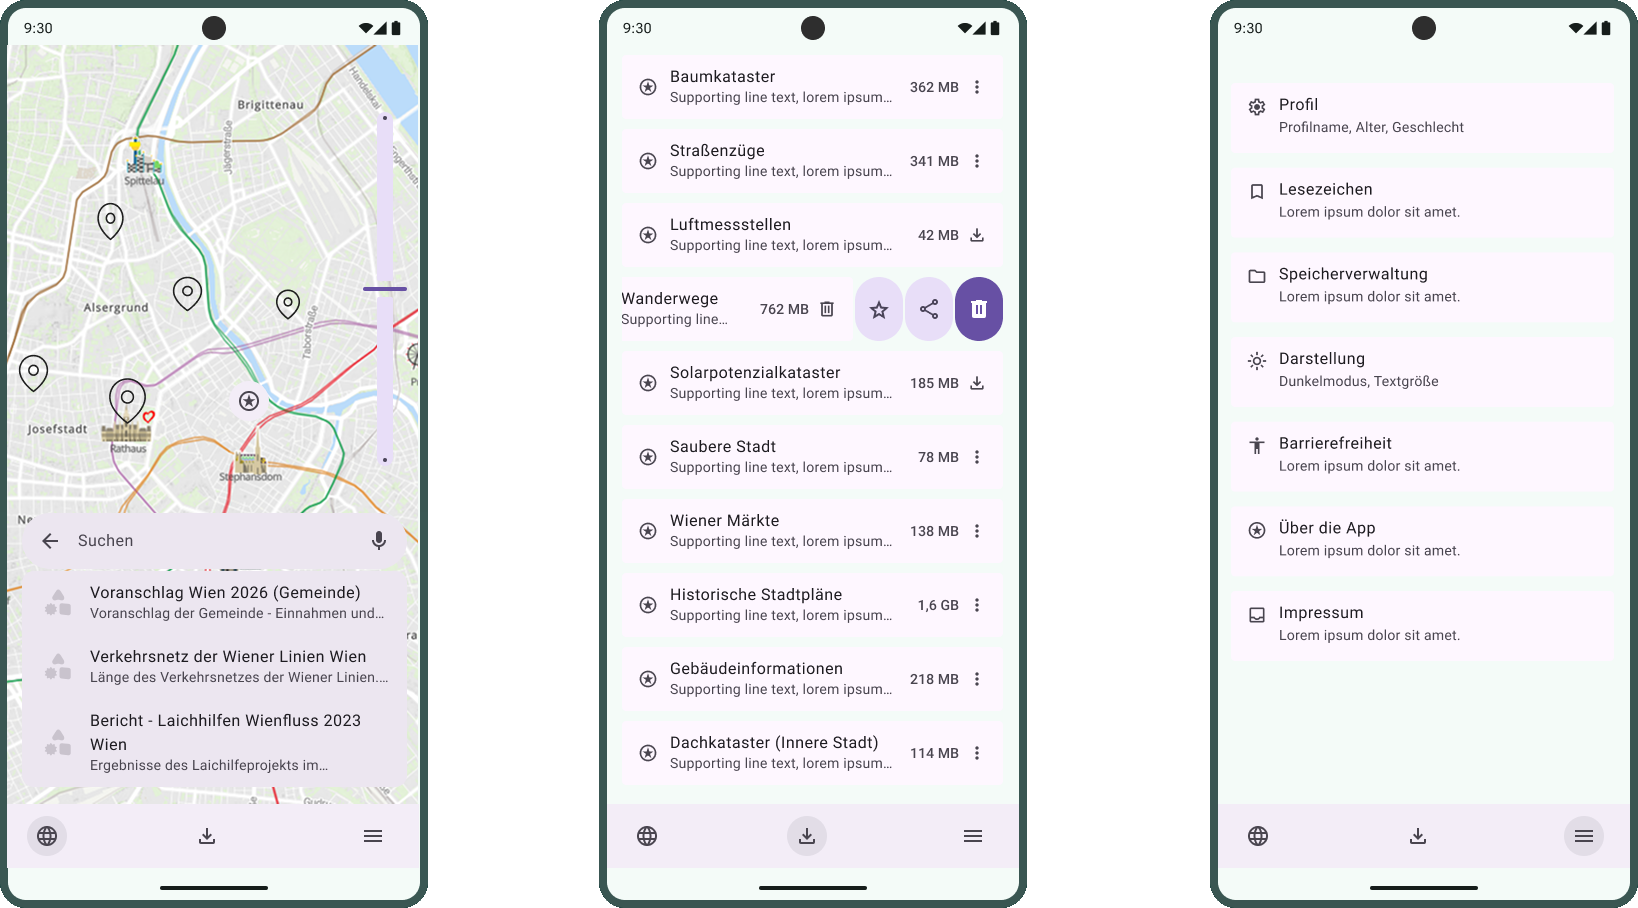
\includegraphics[width=\textwidth]{images/prototype_leonidas.png}
    \end{center}
  \end{frame}
  \begin{frame}{Karte - Anpassung}
    \begin{itemize}
        \item{Benjamin:} Verbesserte Suche
        \item{Leah:} Größe der Pins von Popularität abhängig
    \end{itemize}
  \end{frame}
  \begin{frame}{Evaluierung - Bruder}
  \end{frame}
  \begin{frame}{Evaluierung - KI-Feedback}
    \textbf{St\"{a}rken}
    \begin{itemize}
       \item Gut mit dem Alltag verbindbar
       \item Schönes Design
    \end{itemize}
    \textbf{Schw\"{a}chen}
    \begin{itemize}
        \item Kann unübersichtlich werden
        \item Teils schlechte Namensgebung
    \end{itemize}
  \end{frame}
  \begin{frame}{Story-Explorer Idee}
  \begin{itemize}
    \item Open Data der Stadt Wien soll auch f\"{u}r Menschen ohne technischen Hintergrund verst\"{a}ndlich sein.
    \item Statt isolierter Datens\"{a}tze zeigt die App kurze, leicht lesbare Datenstorys.
    \item Der Ablauf bleibt bewusst einfach: Thema w\"{a}hlen $\rightarrow$ Datensatz w\"{a}hlen $\rightarrow$ Story verstehen.
  \end{itemize}
\end{frame}
%
\begin{frame}{Prototyp - Startseite}
  \centering
  \begin{tikzpicture}
    \node[anchor=center] (img) {%
      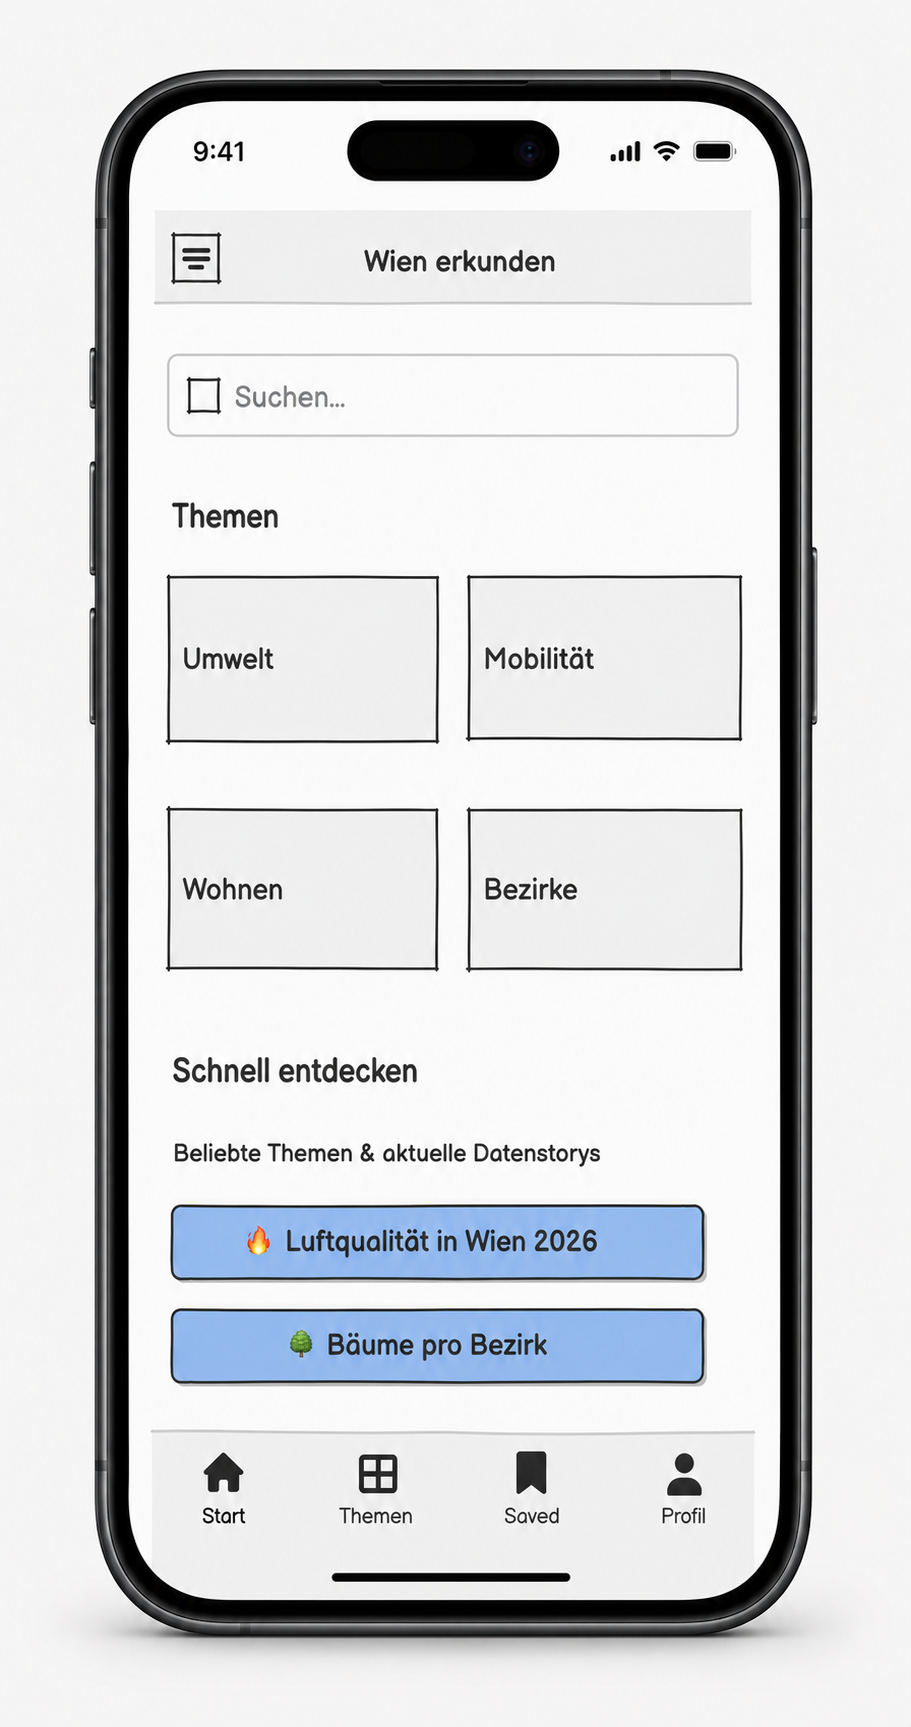
\includegraphics[width=0.90\textwidth,height=0.80\textheight,keepaspectratio]{images/Prototype_1.png}%
    };
    \draw[-{Stealth[scale=1.5]}, orange, line width=2pt]
      ($(img.center)+(-2.5cm, 1.5cm)$) -- ($(img.center)+(-1.0cm, 0.5cm)$)
      node[above left, orange, font=\small\bfseries] at ($(img.center)+(-2.5cm, 1.5cm)$) {Umwelt};
  \end{tikzpicture}
\end{frame}
%
\begin{frame}{Prototyp - Theme\"{u}bersicht}
  \centering
  \begin{tikzpicture}
    \node[anchor=center] (img) {%
      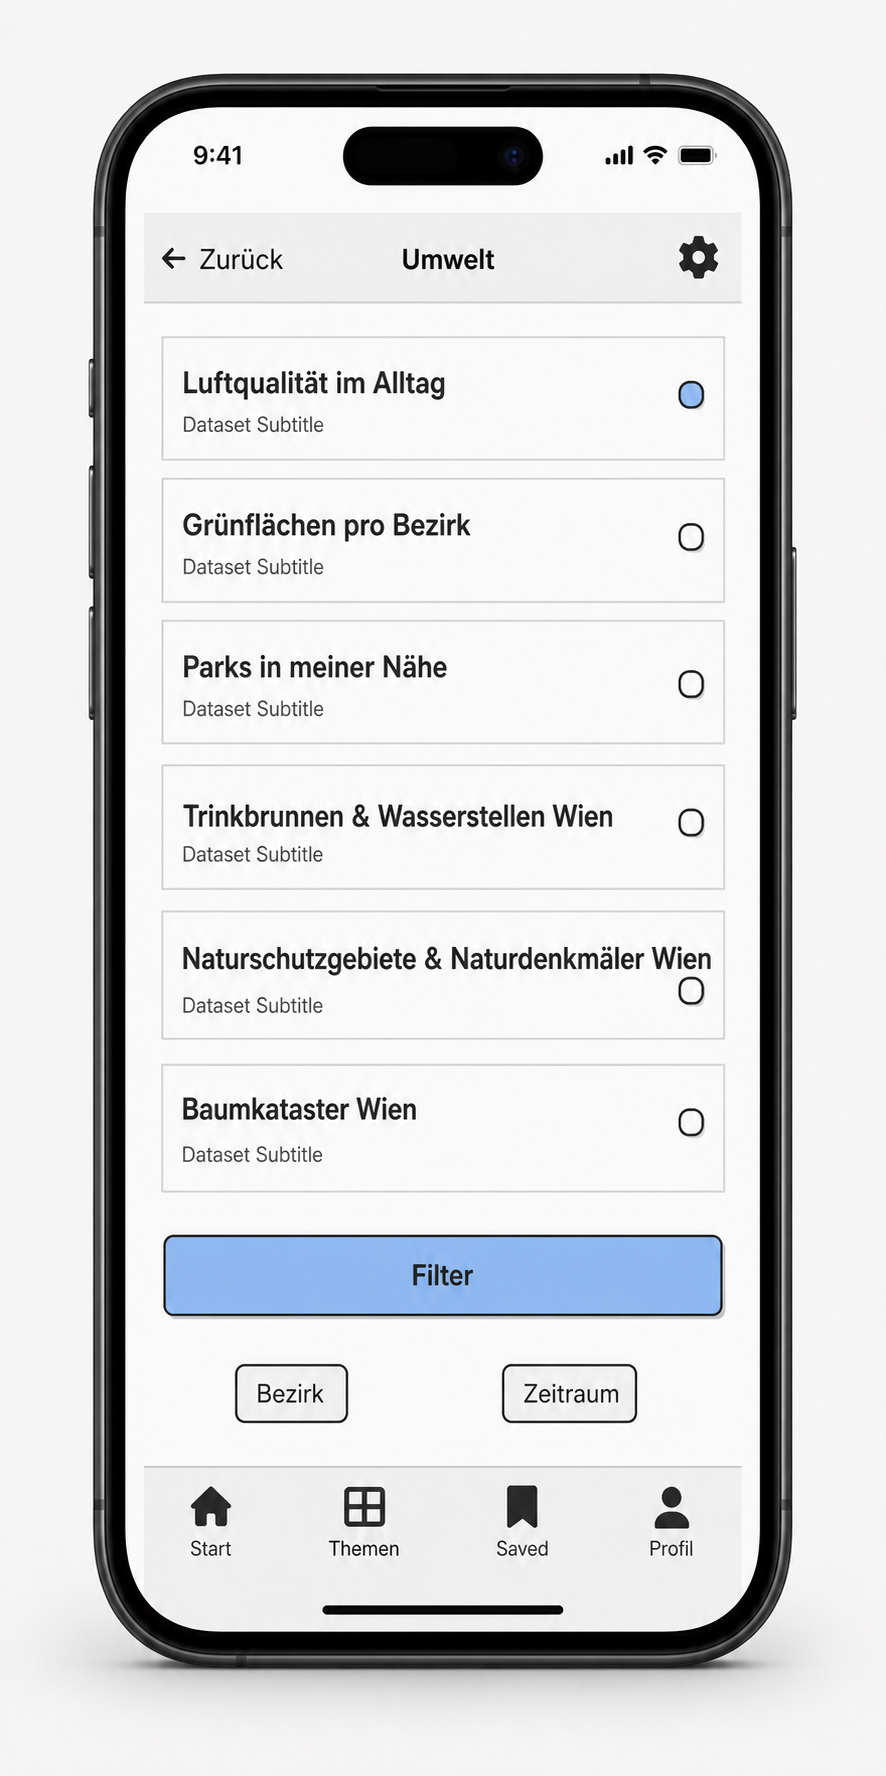
\includegraphics[width=0.90\textwidth,height=0.80\textheight,keepaspectratio]{images/Prototype_2.png}%
    };
    \draw[-{Stealth[scale=1.5]}, orange, line width=2pt]
      ($(img.center)+(-3.2cm, 2.0cm)$) -- ($(img.center)+(-1.3cm, 2.0cm)$);
  \end{tikzpicture}
\end{frame}
%
\begin{frame}{Prototyp - Story-Ansicht}
  \centering
  \begin{tikzpicture}
    \node[anchor=center] (img) {%
      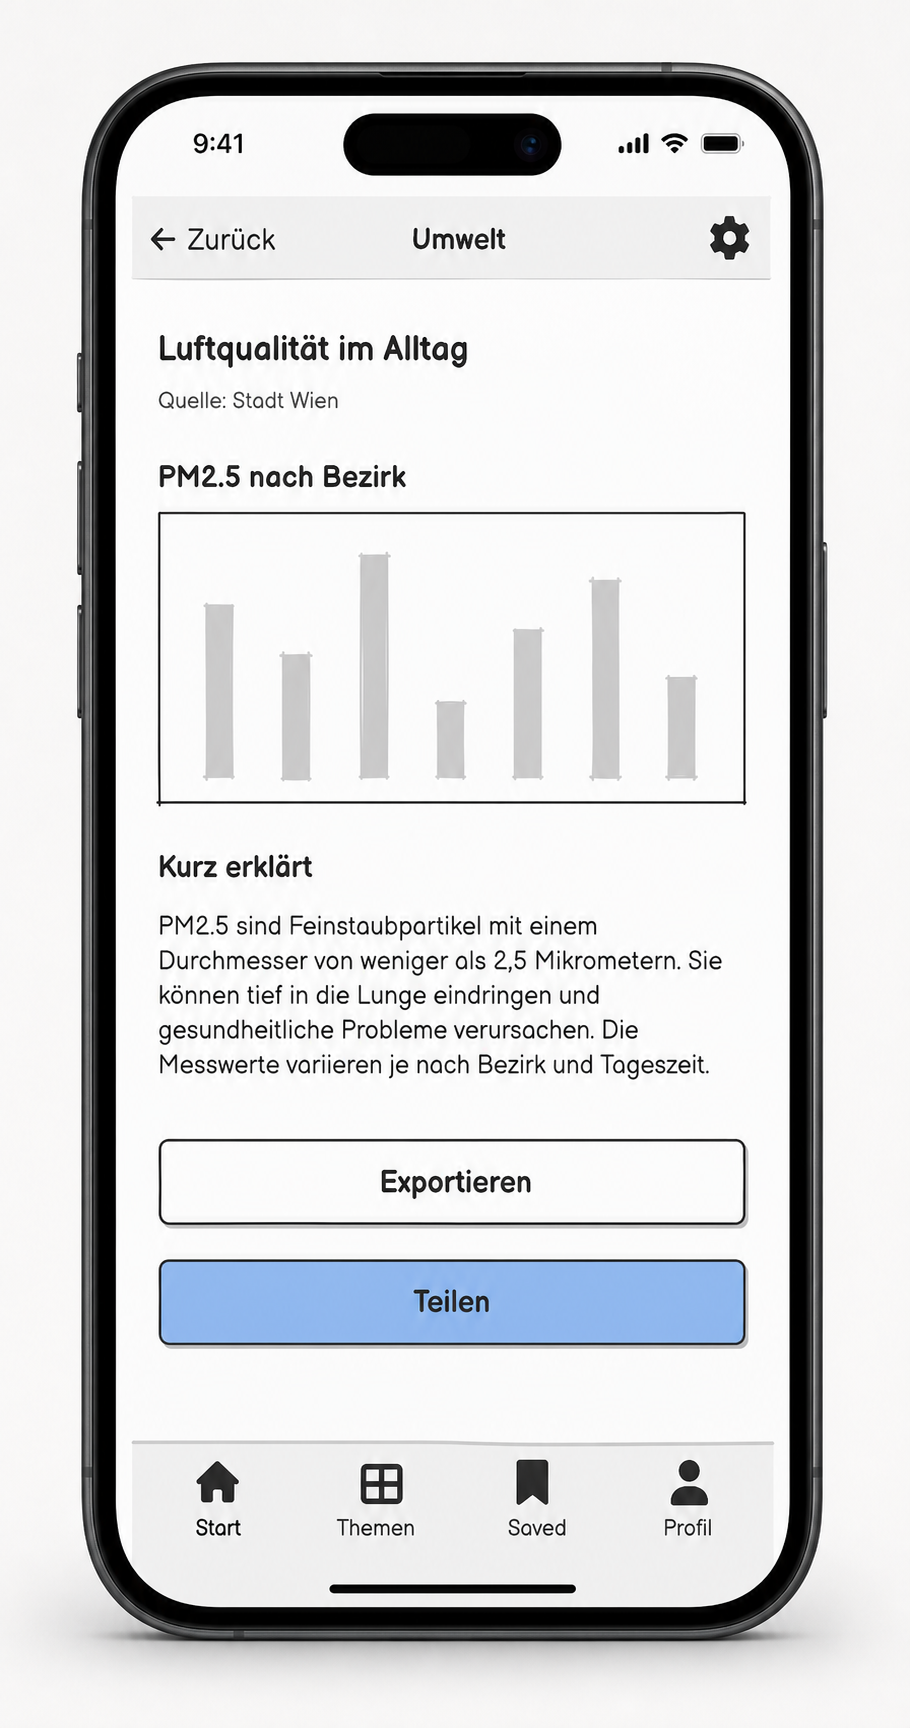
\includegraphics[width=0.90\textwidth,height=0.80\textheight,keepaspectratio]{images/Prototype_3.png}%
    };
  \end{tikzpicture}
\end{frame}
%
\begin{frame}{Anpassung an Personas}
  \begin{itemize}
    \item{Benjamin:} Filter nach Bezirk und Zeitraum f\"{u}r gezielte Suche.
    \item{Leah:} Teilen und Exportieren sind direkt sichtbar.
    \item{Ralph:} Klare Quellenangaben schaffen Transparenz und Vertrauen.
    \item{Luca:} Einfache Einstiege und kurze Erkl\"{a}rungen senken die H\"{u}rde.
  \end{itemize}
\end{frame}
%
\begin{frame}{Evaluierung}
  \begin{block}{Feedback}
    \vspace{0.5em}
    Der klare Ablauf und der ,,Kurz erkl\"{a}rt``-Abschnitt wurde besonders gut gefallen.
  \end{block}

  \vspace{0.5em}
  \textbf{Bevorzugte Kombination:} Story Explorer + Personalisierung von Wien in Zahlen

  \vspace{0.5em}
  \textbf{Verbesserungswunsch:}
  \begin{itemize}
    \item Datens\"{a}tze werden antippbar sein.
  \end{itemize}
\end{frame}

  \begin{frame}{Wien in Zahlen -- Idee}
  \centering

  {\large\bfseries Kurzer Einstieg}\\[-0.2em]
  \rule{0.55\textwidth}{0.4pt}

  \vspace{0.7cm}

  \begin{minipage}{0.78\textwidth}
    \begin{itemize}
      \setlength\itemsep{0.8em}

      \item \textbf{Open Data} als persönlicher Feed statt klassisches Datenportal

      \item \textbf{Kurze Karten} mit verständlichen Datenbeiträgen zu Wien

      \item \textbf{Fact Sheets} mit Visualisierung, Quelle und Alltagsbezug

      \item \textbf{Mitmachen} durch Voting und eigene Fragen

    \end{itemize}
  \end{minipage}

  \vspace{0.6cm}

  {\small
    \textbf{Ziel:} Daten einfach, personalisiert und verständlich vermitteln.
  }

\end{frame}


\begin{frame}{Wien in Zahlen -- Prototyp}
  \centering

  {\large\bfseries Workflow}\\[-0.2em]
  \rule{0.55\textwidth}{0.4pt}

  \vspace{0.45cm}

  \begin{tikzpicture}[
    node distance=0.9cm,
    img/.style={
      inner sep=2pt,
      draw=black!25,
      rounded corners=2pt
    },
    captiontext/.style={
      font=\small,
      align=center
    },
    stepnum/.style={
      font=\scriptsize\bfseries,
      circle,
      draw=black!45,
      inner sep=1.5pt,
      minimum size=0.45cm
    },
    arrow/.style={
      -{Latex[length=3mm]},
      thick,
      black!70
    }
  ]

    % Bilder
    \node[img] (customization) {
      \alt<1->{
        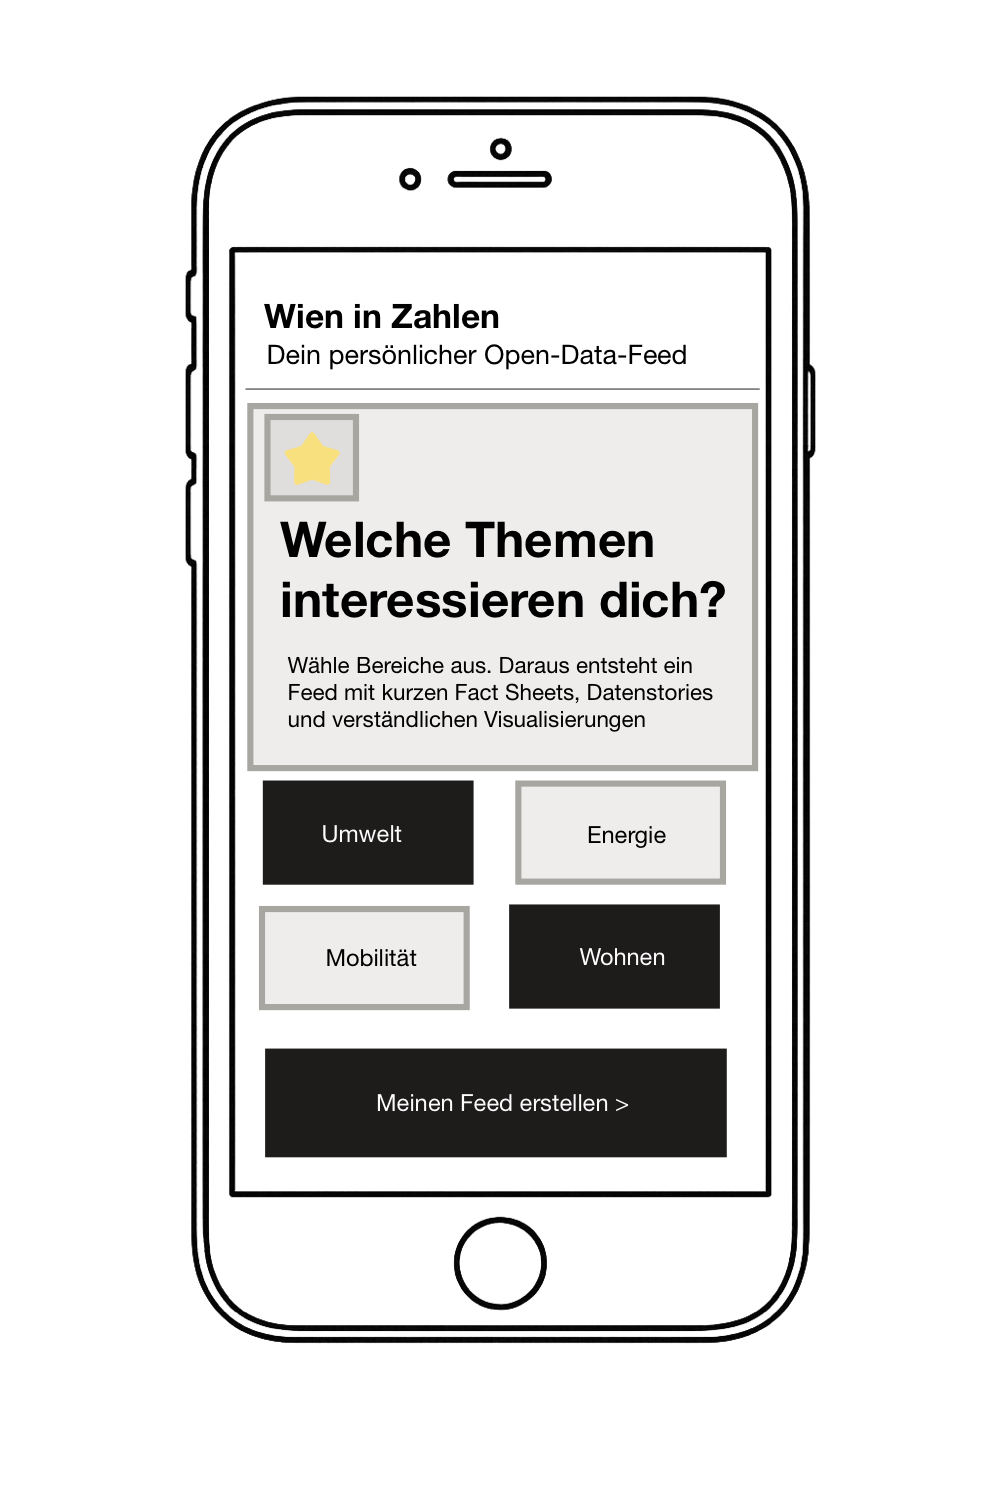
\includegraphics[width=0.25\textwidth]{../milestone_2/images/Feed_auswahl.png}
      }{
        \phantom{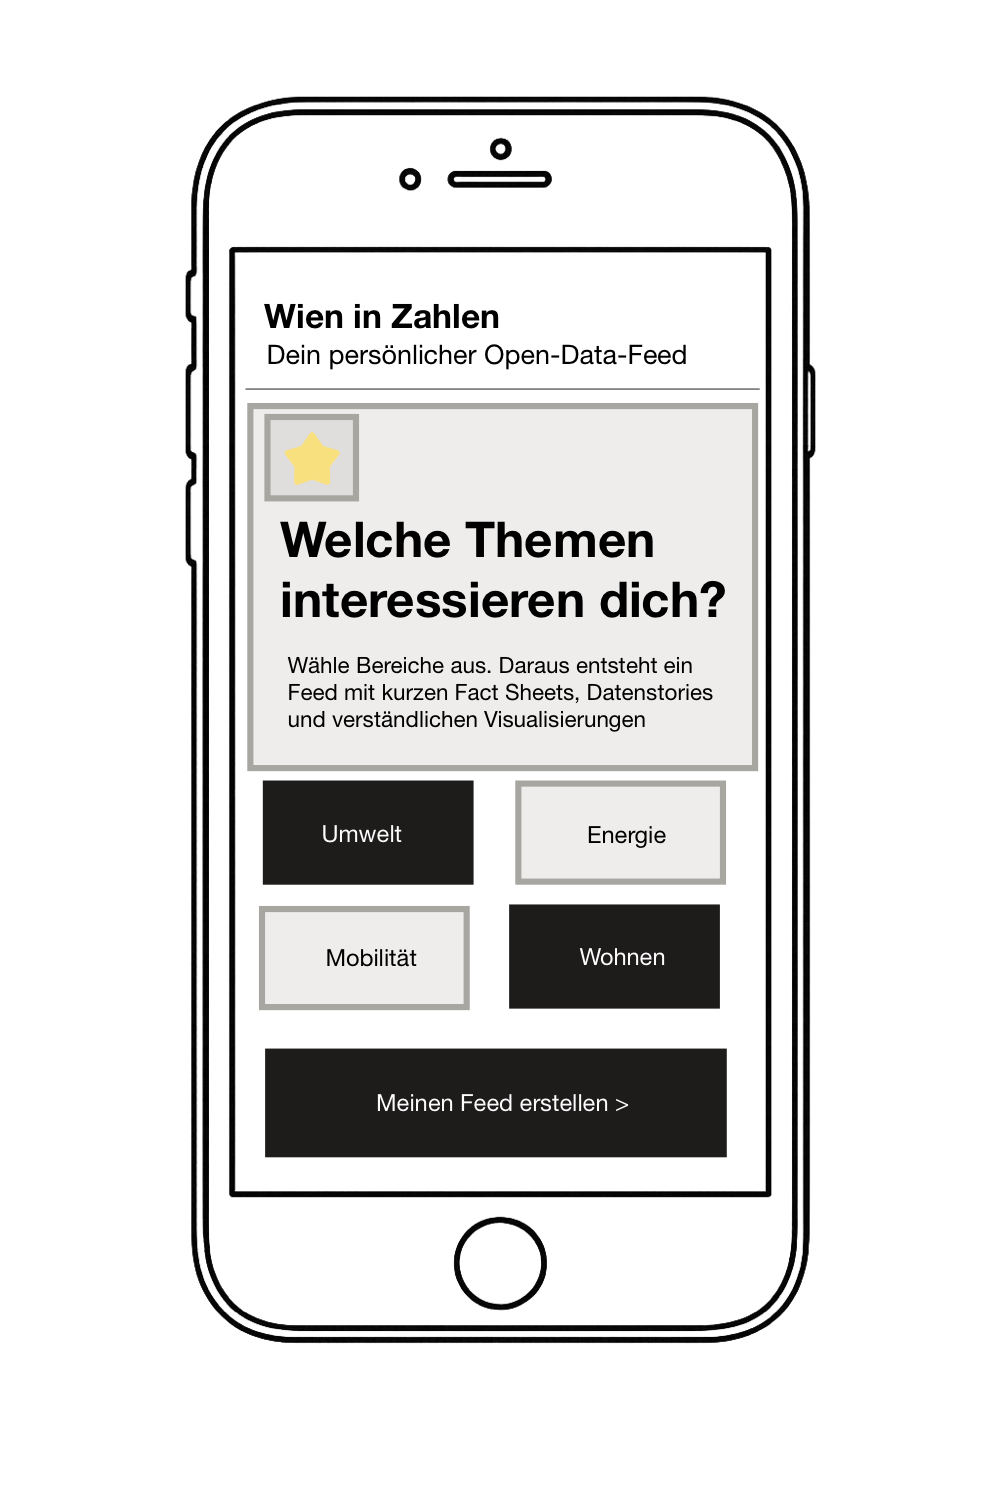
\includegraphics[width=0.25\textwidth]{../milestone_2/images/Feed_auswahl.png}}
      }
    };

    \node[img, right=of customization] (feed) {
      \alt<2->{
        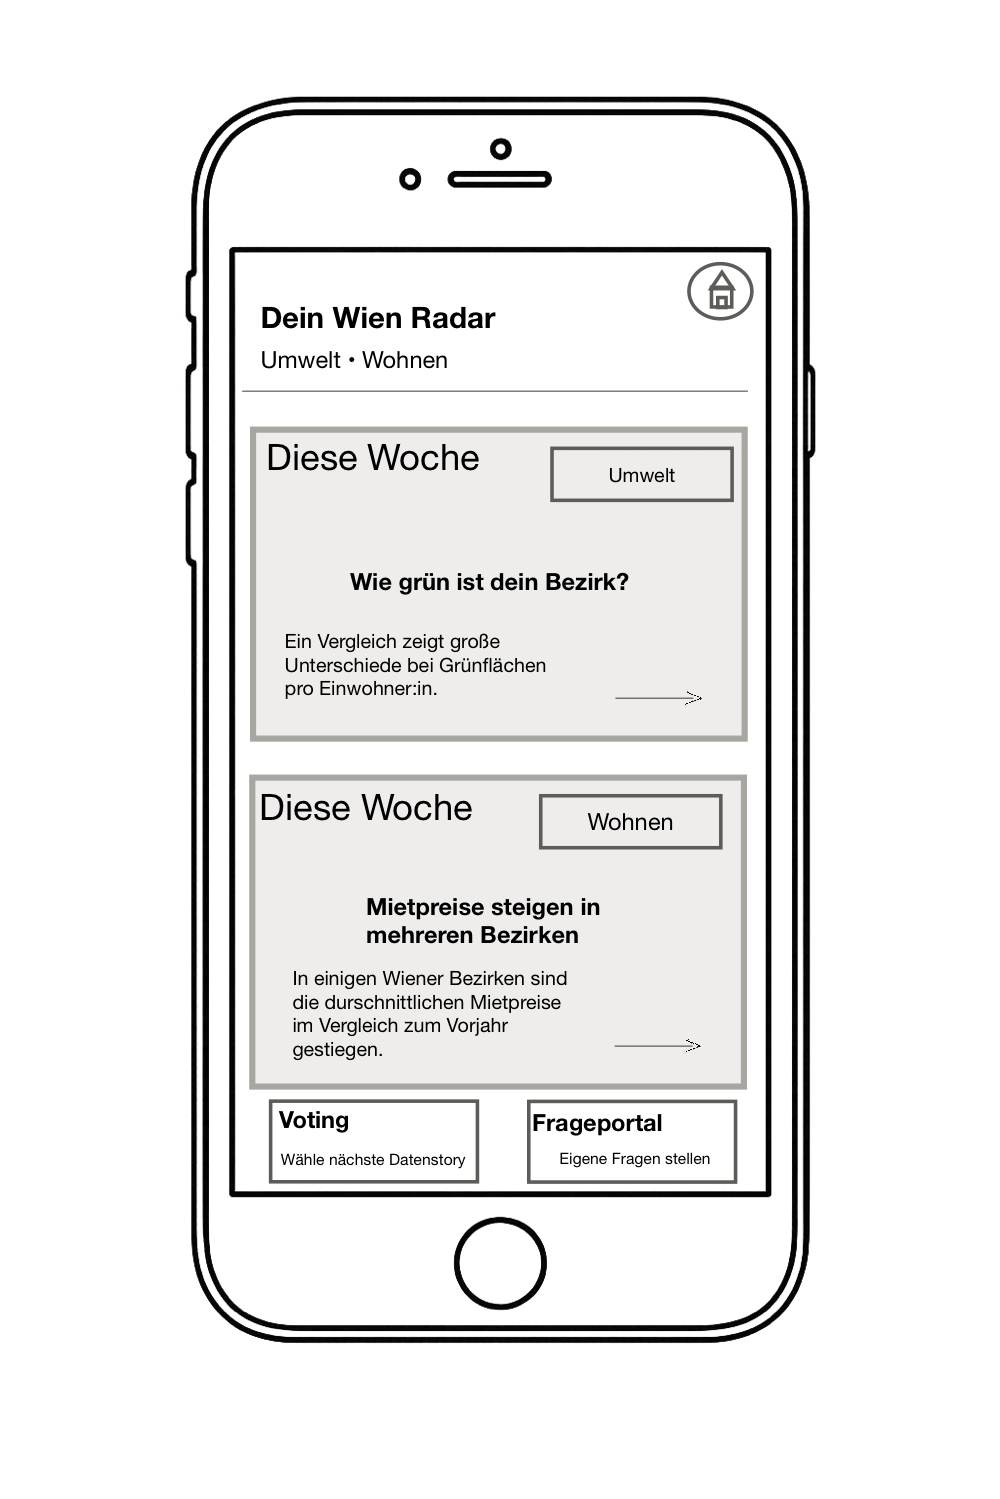
\includegraphics[width=0.25\textwidth]{../milestone_2/images/Feed.png}
      }{
        \phantom{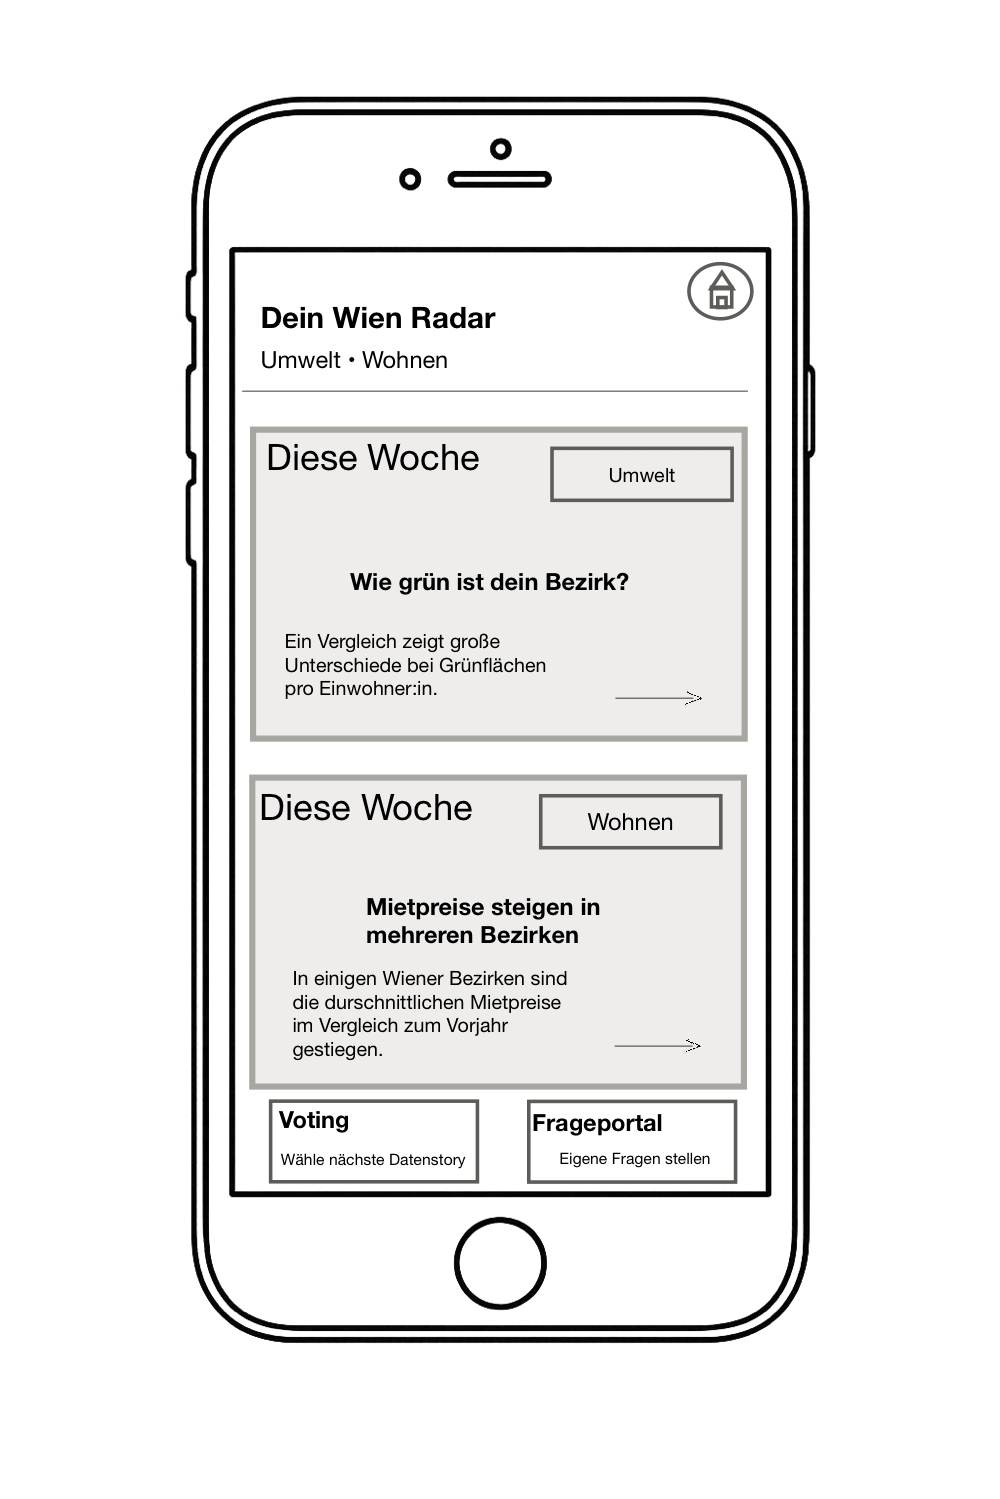
\includegraphics[width=0.25\textwidth]{../milestone_2/images/Feed.png}}
      }
    };

    \node[img, right=of feed] (factsheet) {
      \alt<3->{
        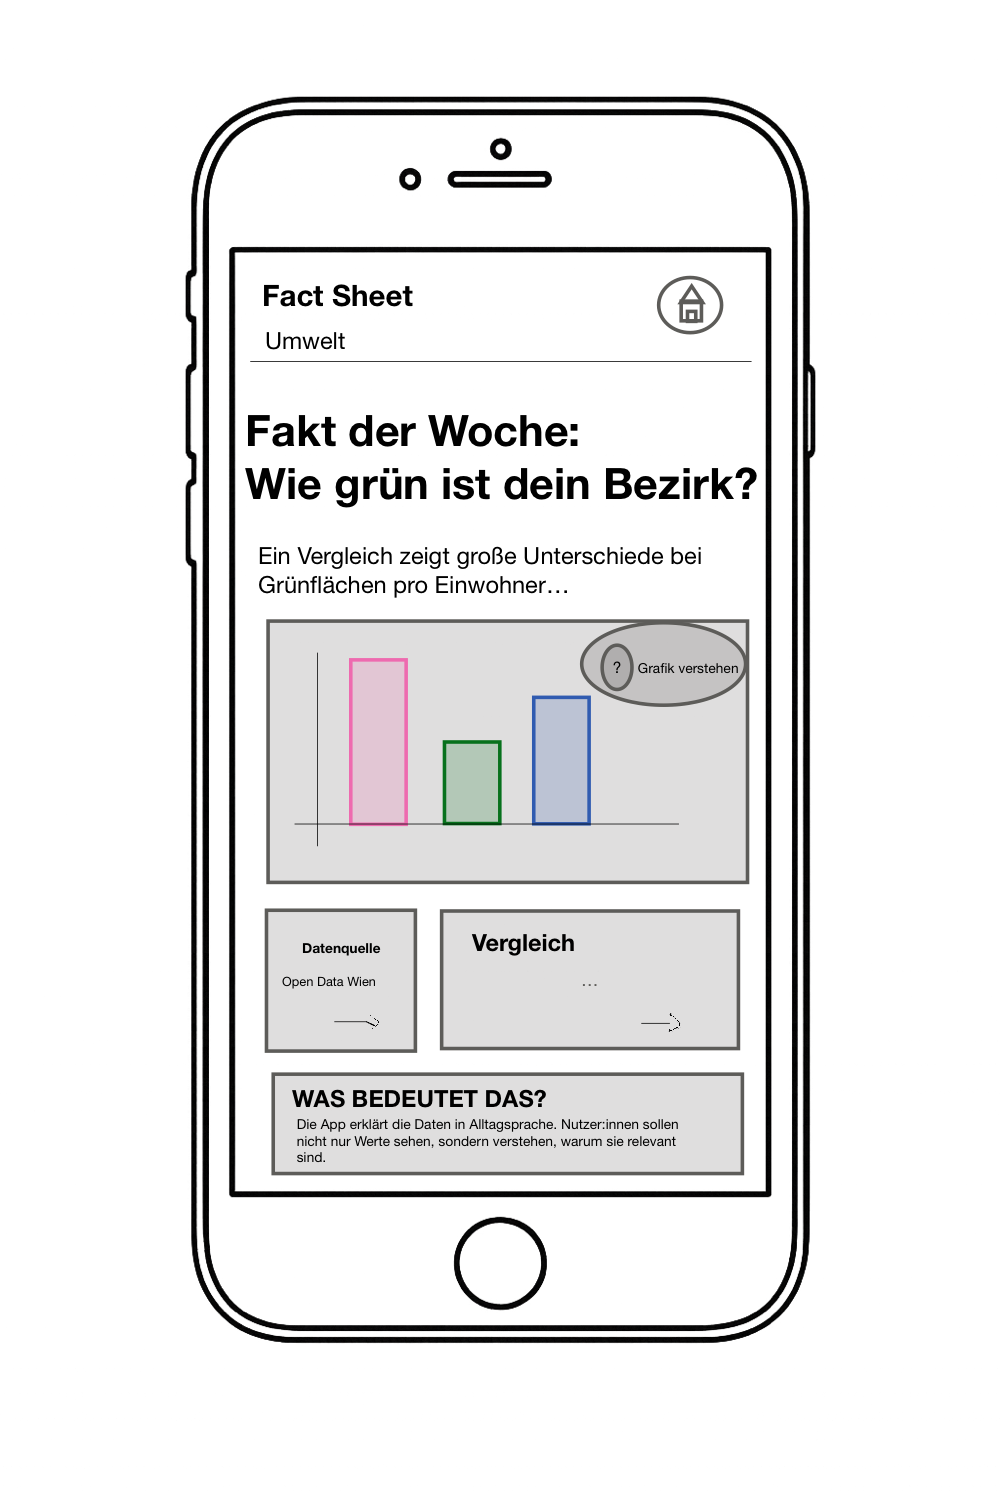
\includegraphics[width=0.25\textwidth]{../milestone_2/images/FactSheet.png}
      }{
        \phantom{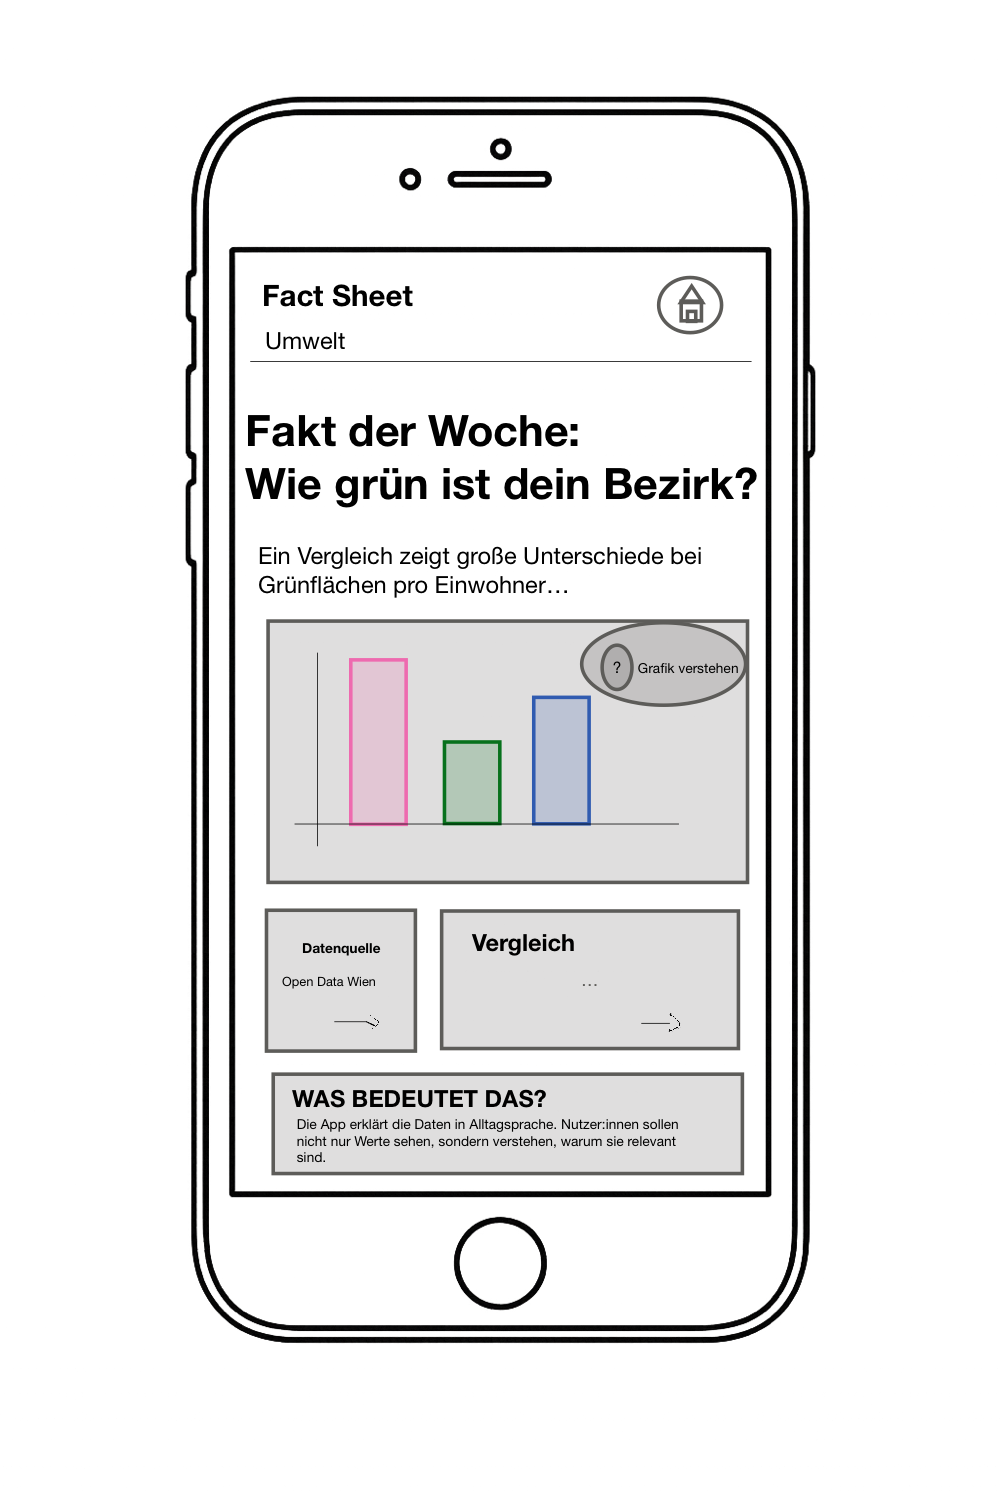
\includegraphics[width=0.25\textwidth]{../milestone_2/images/FactSheet.png}}
      }
    };

    % Pfeile erscheinen ebenfalls schrittweise
    \draw<2->[arrow] (customization.east) -- (feed.west);
    \draw<3->[arrow] (feed.east) -- (factsheet.west);

    % Beschriftungen
    \node[stepnum, below=0.18cm of customization] (s1) {
      \alt<1->{1}{\phantom{1}}
    };
    \node[captiontext, below=0.05cm of s1] {
      \alt<1->{Customization}{\phantom{Customization}}
    };

    \node[stepnum, below=0.18cm of feed] (s2) {
      \alt<2->{2}{\phantom{2}}
    };
    \node[captiontext, below=0.05cm of s2] {
      \alt<2->{Feed}{\phantom{Feed}}
    };

    \node[stepnum, below=0.18cm of factsheet] (s3) {
      \alt<3->{3}{\phantom{3}}
    };
    \node[captiontext, below=0.05cm of s3] {
      \alt<3->{Factsheet}{\phantom{Factsheet}}
    };

  \end{tikzpicture}

\end{frame}

\begin{frame}{Wien in Zahlen -- Anpassung}
  \centering
  \begin{minipage}{0.82\textwidth}
    \begin{itemize}
      \setlength\itemsep{0.85em}

      \item \textbf{Primäre Nutzer:innen:}\\
      Quellen, Vergleiche und Visualisierungen unterstützen Recherche, Analyse und schnelle Weiterverwendung.

      \item \textbf{Sekundäre Nutzer:innen:}\\
      Einfache Bedienung, kurze Texte und Erklärhilfen erleichtern den Einstieg.

      \item \textbf{Negative Persona:}\\
      Kontext, Interpretation und Quellen reduzieren missverständliche Nutzung.

    \end{itemize}
  \end{minipage}

\end{frame}

\begin{frame}{Wien in Zahlen -- Evaluierung}
  \alert{Durchführung:} Mitbewohner die low-Fidelity-Prototypen vorgestellt.

  \vspace{0.4cm}
  \alert{Fazit:}
  \begin{itemize}
    \item Unterschiedliche Zugänge zu Open Data positiv bewertet
    \item Verständlichkeit besonders wichtig
    \item Vertraute Abläufe wie Feed, Karte oder geführte Story hilfreich
  \end{itemize}
\end{frame}
    \begin{frame}{Alexander Prototyp}
    ~2,5min
  \end{frame}
  \section{KI}
    \begin{frame}{Verwendung von KI}
    Künstliche Intelligenz wurde in dieser Arbeit unterstützend verwendet. 
  
    \vspace{0.4cm}
    \begin{itemize}
        \item \textbf{Vincent:} Unterstützung bei TikZ-Code in \LaTeX.
        \item \textbf{Alexander:} ...
        \item \textbf{Leonidas:} ...
        \item \textbf{Neda} ...
    \end{itemize}
\end{frame}
    \begin{frame}{Ende}
    Gibt es noch Fragen, Feeback oder sonstiges?
  \end{frame}
\end{document}
